% answers.tex —— 2002 年·春季京蒙皖卷·理科 · 参考答案与详细解析片段
% 由 tools/generate_projects.py 依来源总账自 2002/2002_数学真题_春季京蒙皖理_试题.md + 2002/2002_数学真题_春季京蒙皖理_解析正文.md + 2002/2002_数学真题_春季京蒙皖理_答案要点.md 生成，勿手改（改源 MD 后重跑）


\begin{gktip}
固定源 PDF 为印刷页码 95–96 的两页题面，不附答案。以下解析均依据题面独立复算；第 15、19 题图形在 LaTeX 工程中以 TikZ/PGFPlots 矢量源重绘。
\end{gktip}

\gkpart{一、选择题}

\begin{answer}
\gksolhead{1}{}

\textbf{题目}：

\Needspace{5\baselineskip}
不等式组

\nopagebreak[4]
\[
\begin{cases}
x^2-1<0,\\
x^2-3x<0
\end{cases}
\]

的解集为\mbox{（　　）}

（A）$\{x\mid -1<x<1\}$　　（B）$\{x\mid 0<x<3\}$

（C）$\{x\mid 0<x<1\}$　　（D）$\{x\mid -1<x<3\}$

\Needspace{4\baselineskip}
\textbf{解析}

两不等式分别给出 $-1<x<1$ 与 $0<x<3$，交集为 $(0,1)$，选 C。

\gkanswer{答案：C。}

\end{answer}
\begin{answer}
\gksolhead{2}{}

\textbf{题目}：

已知三条直线 $m\text{、}n\text{、}l$，三个平面 $\alpha\text{、}\beta\text{、}\gamma$，下列四个命题中，正确的是\mbox{（　　）}

（A）$\begin{cases}\alpha\perp\gamma,\\ \beta\perp\gamma\end{cases}\Rightarrow\alpha\parallel\beta$

（B）$\begin{cases}m\parallel\beta,\\ l\perp m\end{cases}\Rightarrow l\perp\beta$

（C）$\begin{cases}m\parallel\gamma,\\ n\parallel\gamma\end{cases}\Rightarrow m\parallel n$

（D）$\begin{cases}m\perp\gamma,\\ n\perp\gamma\end{cases}\Rightarrow m\parallel n$

\Needspace{4\baselineskip}
\textbf{解析}

两条直线若都垂直于同一平面，则它们平行，故 D 正确。

\gkanswer{答案：D。}

\end{answer}
\begin{answer}
\gksolhead{3}{}

\textbf{题目}：

已知椭圆的焦点是 $F_1\text{、}F_2$，$P$ 是椭圆上的一个动点。如果延长 $F_1P$ 到 $Q$，使得 $|PQ|=|PF_2|$，那么动点 $Q$ 的轨迹是\mbox{（　　）}

（A）圆　　（B）椭圆　　（C）双曲线的一支　　（D）抛物线

\Needspace{4\baselineskip}
\textbf{解析}

由 $F_1Q=F_1P+PQ=F_1P+PF_2=2a$，点 $Q$ 到定点 $F_1$ 的距离恒定，轨迹为圆，选 A。

\gkanswer{答案：A。}

\end{answer}
\begin{answer}
\gksolhead{4}{}

\textbf{题目}：

\Needspace{5\baselineskip}
如果 $\theta\in\left(\dfrac\pi2,\pi\right)$，那么复数

\nopagebreak[4]
\[
(1+i)(\cos\theta+i\sin\theta)
\]

的辐角的主值是\mbox{（　　）}

（A）$\theta+\dfrac{9\pi}{4}$　　（B）$\theta+\dfrac\pi4$　　（C）$\theta-\dfrac\pi4$　　（D）$\theta+\dfrac{7\pi}{4}$

\Needspace{4\baselineskip}
\textbf{解析}

乘积的辐角为 $\theta+\pi/4$，且该值属于主值范围，选 B。

\gkanswer{答案：B。}

\end{answer}
\begin{answer}
\gksolhead{5}{}

\textbf{题目}：

若角 $\alpha$ 满足 $\sin2\alpha<0$，$\cos\alpha-\sin\alpha<0$，则 $\alpha$ 在\mbox{（　　）}

（A）第一象限　　（B）第二象限　　（C）第三象限　　（D）第四象限

\Needspace{4\baselineskip}
\textbf{解析}

$\sin2\alpha<0$ 给出第二或第四象限；只有第二象限满足 $\cos\alpha-\sin\alpha<0$，选 B。

\gkanswer{答案：B。}

\end{answer}
\begin{answer}
\gksolhead{6}{}

\textbf{题目}：

从 6 名志愿者中选出 4 人分别从事翻译、导游、导购、保洁四项不同工作。若其中甲、乙两名志愿者都不能从事翻译工作，则选派方案共有\mbox{（　　）}

（A）280 种　　（B）240 种　　（C）180 种　　（D）96 种

\Needspace{4\baselineskip}
\textbf{解析}

翻译工作有 $4$ 种人选，其他三项从剩余 5 人中排列，方案数为 $4P_5^3=240$，选 B。

\gkanswer{答案：B。}

\end{answer}
\begin{answer}
\gksolhead{7}{}

\textbf{题目}：

在 $\triangle ABC$ 中，$AB=2$，$BC=1.5$，$\angle ABC=120^\circ$。若使三角形绕直线 $BC$ 旋转一周，则所形成的几何体的体积是\mbox{（　　）}

（A）$\dfrac32\pi$　　（B）$\dfrac52\pi$　　（C）$\dfrac72\pi$　　（D）$\dfrac92\pi$

\Needspace{4\baselineskip}
\textbf{解析}

\Needspace{5\baselineskip}
旋转所得为半径 $AB\sin120^\circ=\sqrt3$、高 $BC=1.5$ 的圆锥，体积为

\nopagebreak[4]
\[
\frac13\pi(\sqrt3)^2\cdot1.5=\frac32\pi,
\]

选 A。

\gkanswer{答案：A。}

\end{answer}
\begin{answer}
\gksolhead{8}{}

\textbf{题目}：

\Needspace{5\baselineskip}
圆 $2x^2+2y^2=1$ 与直线

\nopagebreak[4]
\[
x\sin\theta+y-1=0
\qquad\left(\theta\in\mathbb R,\ \theta\ne\frac\pi2+k\pi,\ k\in\mathbb Z\right)
\]

的位置关系是\mbox{（　　）}

（A）相交　　（B）相切　　（C）相离或相切　　（D）不能确定

\Needspace{4\baselineskip}
\textbf{解析}

\Needspace{5\baselineskip}
圆心为原点、半径 $1/\sqrt2$。直线到原点的距离为

\nopagebreak[4]
\[
\frac1{\sqrt{1+\sin^2\theta}}.
\]

因 $\theta\ne\pi/2+k\pi$，有 $0<|\sin\theta|\le1$，该距离在 $1/\sqrt2$ 与 $1$ 之间，故直线可能相切或相离，选 C。

\gkanswer{答案：C。}

\end{answer}
\begin{answer}
\gksolhead{9}{}

\textbf{题目}：

\Needspace{5\baselineskip}
在极坐标系中，如果一个圆的方程

\nopagebreak[4]
\[
\rho=4\cos\theta+6\sin\theta,
\]

那么过圆心且与极轴平行的直线方程是\mbox{（　　）}

（A）$\rho\sin\theta=3$　　（B）$\rho\sin\theta=-3$　　（C）$\rho\cos\theta=2$　　（D）$\rho\cos\theta=-2$

\Needspace{4\baselineskip}
\textbf{解析}

\Needspace{5\baselineskip}
极坐标方程化为

\nopagebreak[4]
\[
\rho^2-4\rho\cos\theta-6\rho\sin\theta=0,
\]

即圆心笛卡尔坐标为 $(2,3)$。过圆心且平行于极轴的直线为 $y=3$，即 $\rho\sin\theta=3$，选 A。

\gkanswer{答案：A。}

\end{answer}
\begin{answer}
\gksolhead{10}{}

\textbf{题目}：

\Needspace{5\baselineskip}
对于二项式

\nopagebreak[4]
\[
\left(\frac1x+x^3\right)^n\qquad(n\in\mathbb N^*),
\]

四位同学作出了四种判断：

① 存在 $n\in\mathbb N^*$，展开式中有常数项；

② 对任意 $n\in\mathbb N^*$，展开式中没有常数项；

③ 对任意 $n\in\mathbb N^*$，展开式中没有 $x$ 的一次项；

④ 存在 $n\in\mathbb N^*$，展开式中有 $x$ 的一次项。

上述判断中正确的是\mbox{（　　）}

（A）①与③　　（B）②与③　　（C）①与④　　（D）②与④

\Needspace{4\baselineskip}
\textbf{解析}

\Needspace{5\baselineskip}
通项的幂为

\nopagebreak[4]
\[
-n+4r.
\]

存在常数项当且仅当 $n$ 是 4 的倍数，因此 ①正确；存在一次项当且仅当 $n\equiv3\pmod4$，因此 ④正确。选 C。

\gkanswer{答案：C。}

\end{answer}
\begin{answer}
\gksolhead{11}{}

\textbf{题目}：

若一个等差数列前 3 项的和为 34，最后 3 项的和为 146，且所有项的和为 390，则这个数列有\mbox{（　　）}

（A）13 项　　（B）12 项　　（C）11 项　　（D）10 项

\Needspace{4\baselineskip}
\textbf{解析}

前 3 项和与最后 3 项和的平均分别为 $34/3$、$146/3$，故首末项之和为 $60$。总和为 $390$，所以 $30n=390$，得 $n=13$，选 A。

\gkanswer{答案：A。}

\end{answer}
\begin{answer}
\gksolhead{12}{}

\textbf{题目}：

用一张钢板制作一个容积为 $4\text{ m}^3$ 的无盖长方体水箱。可用的长方形钢板有四种不同的规格（长$\times$宽的尺寸如各选项所示，单位均为 m），若既要够用，又要所剩最少，则应选钢板的规格是\mbox{（　　）}

（A）$2\times5$　　（B）$2\times5.5$　　（C）$2\times6.1$　　（D）$3\times5$

\Needspace{4\baselineskip}
\textbf{解析}

容积为 $4\text{ m}^3$ 的无盖长方体所需最小表面积为 $12\text{ m}^2$。四种钢板中 $2\times6.1$ 是面积刚好够且剩余最少的规格，选 C。

\gkanswer{答案：C。}

\end{answer}
\gkpart{二、填空题}

\begin{answer}
\gksolhead{13}{}

\textbf{题目}：

\Needspace{5\baselineskip}
若双曲线

\nopagebreak[4]
\[
\frac{x^2}{4}-\frac{y^2}{m}=1
\]

的渐近线方程为 $y=\pm\dfrac{\sqrt3}{2}x$，则双曲线的焦点坐标是\gkblank{}。

\Needspace{4\baselineskip}
\textbf{解析}

由渐近线斜率 $b/a=\sqrt3/2$ 与 $a=2$，得 $b^2=m=3$。故 $c^2=a^2+b^2=7$，焦点为 $(\pm\sqrt7,0)$。

\gkanswer{答案：$(\pm\sqrt7,0)$。}

\end{answer}
\begin{answer}
\gksolhead{14}{}

\textbf{题目}：

\Needspace{5\baselineskip}
如果 $\cos\theta=-\dfrac{12}{13}$，$\theta\in\left(\pi,\dfrac{3\pi}{2}\right)$，那么

\nopagebreak[4]
\[
\cos\left(\theta+\frac{3\pi}{4}\right)
\]

的值等于\gkblank{}。

\Needspace{4\baselineskip}
\textbf{解析}

\Needspace{5\baselineskip}
在第三象限，$\sin\theta=-5/13$。因此

\nopagebreak[4]
\[
\cos\left(\theta+\frac{3\pi}{4}\right)
=\frac{17\sqrt2}{26}.
\]

\gkanswer{答案：$\dfrac{17\sqrt2}{26}$。}

\end{answer}
\begin{answer}
\gksolhead{15}{}

\textbf{题目}：

正方形 $ABCD$ 的边长是 2，$E\text{、}F$ 分别是 $AB$ 和 $CD$ 的中点，将正方形沿 $EF$ 折成直二面角（如图所示）。$M$ 为矩形 $AEFD$ 内一点，如果 $\angle MBE=\angle MBC$，$MB$ 和平面 $BCF$ 所成角的正切值为 $\dfrac12$，那么点 $M$ 到直线 $EF$ 的距离为\gkblank{}。
\nopagebreak[4]
\begin{center}% 2002 年春季京蒙皖理卷第 15 题：正方形折叠成直二面角
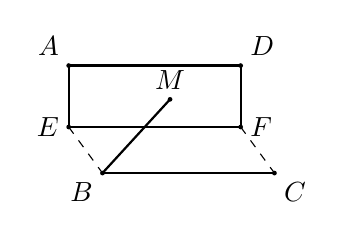
\begin{tikzpicture}[scale=0.78]
  \coordinate (A) at (0,2);
  \coordinate (D) at (2.8,2);
  \coordinate (E) at (0,1);
  \coordinate (F) at (2.8,1);
  \coordinate (B) at (0.55,0.25);
  \coordinate (C) at (3.35,0.25);
  \coordinate (M) at (1.65,1.45);

  \draw[thick] (A)--(D)--(F)--(E)--cycle;
  \draw[thick] (E)--(F);
  \draw[thick] (B)--(C);
  \draw[dashed] (E)--(B) (F)--(C);
  \draw[thick] (B)--(M);

  \fill (A) circle (1.1pt) node[above left] {$A$};
  \fill (D) circle (1.1pt) node[above right] {$D$};
  \fill (E) circle (1.1pt) node[left] {$E$};
  \fill (F) circle (1.1pt) node[right] {$F$};
  \fill (B) circle (1.1pt) node[below left] {$B$};
  \fill (C) circle (1.1pt) node[below right] {$C$};
  \fill (M) circle (1.1pt) node[above] {$M$};
\end{tikzpicture}
\end{center}
\nopagebreak[4]
\Needspace{4\baselineskip}
\textbf{解析}

\Needspace{5\baselineskip}
取

\nopagebreak[4]
\[
E=(0,0,0),\ F=(2,0,0),\ A=(0,1,0),\ D=(2,1,0),
\]

\nopagebreak[4]
\[
B=(0,0,-1),\ C=(2,0,-1),\ M=(u,v,0).
\]

\Needspace{5\baselineskip}
由 $\angle MBE=\angle MBC$ 得 $u=1$。又

\nopagebreak[4]
\[
\tan\angle(MB,\text{\text{平面} }BCF)=\frac v{\sqrt2}=\frac12,
\]

所以 $v=\sqrt2/2$，即点 $M$ 到 $EF$ 的距离为 $\sqrt2/2$。

\gkanswer{答案：$\dfrac{\sqrt2}{2}$。}

\end{answer}
\begin{answer}
\gksolhead{16}{}

\textbf{题目}：

\Needspace{5\baselineskip}
对于任意两个复数 $z_1=x_1+y_1i$、$z_2=x_2+y_2i$（$x_1\text{、}y_1\text{、}x_2\text{、}y_2$ 为实数），定义运算 $\odot$ 为

\nopagebreak[4]
\[
z_1\odot z_2=x_1x_2+y_1y_2.
\]

设非零复数 $w_1\text{、}w_2$ 在复平面内对应的点分别为 $P_1\text{、}P_2$，点 $O$ 为坐标原点。如果 $w_1\odot w_2=0$，那么在 $\triangle P_1OP_2$ 中，$\angle P_1OP_2$ 的大小为\gkblank{}。

\Needspace{4\baselineskip}
\textbf{解析}

$w_1\odot w_2=0$ 表示对应的两个平面向量内积为零，故 $\angle P_1OP_2=90^\circ$。

\gkanswer{答案：$90^\circ$。}

\end{answer}
\gkpart{三、解答题}

\begin{answer}
\gksolhead{17}{}

\textbf{题目}：

\Needspace{5\baselineskip}
在 $\triangle ABC$ 中，已知 $A\text{、}B\text{、}C$ 成等差数列，求

\nopagebreak[4]
\[
\tan\frac A2+\tan\frac C2+\sqrt3\tan\frac A2\tan\frac C2
\]

的值。

\Needspace{4\baselineskip}
\textbf{解析}

\Needspace{5\baselineskip}
由 $A\text{、}B\text{、}C$ 成等差数列且和为 $\pi$，得 $B=\pi/3$、$A+C=2\pi/3$。令 $x=\tan(A/2)$、$y=\tan(C/2)$，则

\nopagebreak[4]
\[
\frac{x+y}{1-xy}=\sqrt3,
\]

所求式为 $\sqrt3$。

\gkanswer{答案：$\sqrt3$。}

\end{answer}
\begin{answer}
\gksolhead{18}{}

\textbf{题目}：

已知函数 $f(x)$ 是偶函数，而且在 $(0,+\infty)$ 上是增函数，判断 $f(x)$ 在 $(-\infty,0)$ 上是增函数还是减函数，并证明你的判断。

\Needspace{4\baselineskip}
\textbf{解析}

\Needspace{5\baselineskip}
若 $x_1<x_2<0$，则 $-x_1>-x_2>0$。由偶性和正半轴上的增性，

\nopagebreak[4]
\[
f(x_1)=f(-x_1)>f(-x_2)=f(x_2),
\]

故负半轴上为减函数。

\gkanswer{答案：在 $(-\infty,0)$ 上为减函数。}

\end{answer}
\begin{answer}
\gksolhead{19}{}

\textbf{题目}：

在三棱锥 $S-ABC$ 中，如图，$\angle SAB=\angle SAC=\angle ACB=90^\circ$，$AC=2$，$BC=\sqrt{13}$，$SB=\sqrt{29}$。
\nopagebreak[4]
\begin{center}% 2002 年春季京蒙皖理卷第 19 题：三棱锥空间图形
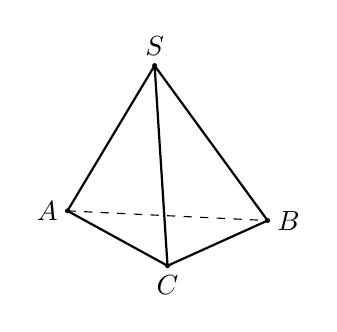
\begin{tikzpicture}[>=stealth, scale=0.82]
  \coordinate (A) at (0,0);
  \coordinate (C) at (1.55,-0.85);
  \coordinate (B) at (3.1,-0.15);
  \coordinate (S) at (1.35,2.25);

  \draw[thick] (A)--(C)--(B);
  \draw[dashed] (A)--(B);
  \draw[thick] (S)--(A) (S)--(B) (S)--(C);

  \fill (A) circle (1.1pt) node[left] {$A$};
  \fill (B) circle (1.1pt) node[right] {$B$};
  \fill (C) circle (1.1pt) node[below] {$C$};
  \fill (S) circle (1.1pt) node[above] {$S$};
\end{tikzpicture}
\end{center}
\nopagebreak[4]
（1） 证明：$SC\perp BC$；

（2） 求侧面 $SBC$ 与底面 $ABC$ 所成的二面角大小；

（3） 求异面直线 $SC$ 与 $AB$ 所成的角的大小（用反三角函数表示）。

\Needspace{4\baselineskip}
\textbf{解析}

\Needspace{5\baselineskip}
取

\nopagebreak[4]
\[
A=(0,0,0),\quad C=(0,2,0),\quad B=(\sqrt{13},2,0),\quad S=(0,0,2\sqrt3).
\]

由 $SB^2=13+4+12=29$，坐标满足题设。

\gksubpart{(1)}

\nopagebreak[4]
\[
\overrightarrow{SC}=(0,2,-2\sqrt3),\qquad
\overrightarrow{BC}=(-\sqrt{13},0,0),
\]

内积为零，故 $SC\perp BC$。

\gksubpart{(2)}

平面 $ABC$ 的法向量为 $(0,0,1)$；平面 $SBC$ 的法向量可由 $\overrightarrow{CB}\times\overrightarrow{CS}$ 得到。两法向量夹角的余弦为 $1/2$，故二面角为 $\pi/3$。

\gksubpart{(3)}

\Needspace{5\baselineskip}
取 $\overrightarrow{SC}$ 与 $\overrightarrow{AB}=(\sqrt{13},2,0)$，则

\nopagebreak[4]
\[
\frac{|\overrightarrow{SC}\cdot\overrightarrow{AB}|}
{|\overrightarrow{SC}|\,|\overrightarrow{AB}|}
=\frac1{\sqrt{17}}.
\]

\Needspace{5\baselineskip}
故异面直线所成角为 $\arccos(1/\sqrt{17})$。

\nopagebreak[4]
\[
\text{（1） }SC\perp BC;\qquad
\text{（2） }\frac\pi3;\qquad
\text{（3） }\arccos\frac1{\sqrt{17}}.
\]

\gkanswer{答案（1）：见解析。}

\gkanswer{答案（2）：$\dfrac\pi3$。}

\gkanswer{答案（3）：$\arccos\dfrac1{\sqrt{17}}$。}

\end{answer}
\begin{answer}
\gksolhead{20}{}

\textbf{题目}：

假设 A 型进口车关税税率在 2001 年是 100\%，在 2006 年是 25\%，2001 年 A 型进口车每辆价格为 64 万元（其中含 32 万元关税税款）。

（1） 已知与 A 型车性能相近的 B 型国产车，2001 年每辆价格为 46 万元。若 A 型车的价格只受关税降低的影响，为了保证 2006 年 B 型车的价格不高于 A 型车价格的 90\%，B 型车价格要逐年降低，问平均每年至少下降多少万元？

（2） 某人在 2001 年将 33 万元存入银行，假设银行扣利息税后的年利率为 1.8\%（5 年内不变），且每年按复利计算（上一年的利息计入第二年的本金），那么五年到期时这笔钱连本带息是否一定够买按（1）中所述降价后的 B 型车一辆？

\Needspace{4\baselineskip}
\textbf{解析}

\gksubpart{(1)}

A 型车 2006 年价格为 $32(1+25\%)=40$ 万元，B 型车目标上限为 $36$ 万元，所以平均每年至少下降 $(46-36)/5=2$ 万元。

\gksubpart{(2)}

\Needspace{5\baselineskip}
某人在 2001 年存入的 33 万元五年后本息为

\nopagebreak[4]
\[
33(1.018)^5\approx36.08>36,
\]

故五年本息一定够买降价后的 B 型车。

\gkanswer{答案（1）：平均每年至少下降 $2$ 万元。}

\gkanswer{答案（2）：一定够买。}

\end{answer}
\begin{answer}
\gksolhead{21}{}

\textbf{题目}：

已知点的序列 $A_n(x_n,0)$，$n\in\mathbb N$，其中 $x_1=0$，$x_2=a$（$a<0$），$A_3$ 是线段 $A_1A_2$ 的中点，$A_4$ 是线段 $A_2A_3$ 的中点，$\cdots$，$A_n$ 是线段 $A_{n-2}A_{n-1}$ 的中点，$\cdots$。

（1） 写出 $x_n$ 与 $x_{n-1}\text{、}x_{n-2}$ 之间的关系式（$n\ge3$）；

（2） 设 $a_n=x_{n+1}-x_n$，计算 $a_1\text{、}a_2\text{、}a_3$，由此推测数列 $\{a_n\}$ 的通项公式，并加以证明；

（3） 求 $\displaystyle\lim_{n\to\infty}x_n$。

\Needspace{4\baselineskip}
\textbf{解析}

\gksubpart{(1)}

\Needspace{5\baselineskip}
由中点定义

\nopagebreak[4]
\[
x_n=\frac{x_{n-1}+x_{n-2}}2.
\]

\gksubpart{(2)}

\Needspace{5\baselineskip}
令 $a_n=x_{n+1}-x_n$，则 $a_n=-a_{n-1}/2$。因此

\nopagebreak[4]
\[
a_1=a,\quad a_2=-\frac a2,\quad a_3=\frac a4,\quad
a_n=a\left(-\frac12\right)^{n-1}.
\]

\gksubpart{(3)}

\Needspace{5\baselineskip}
求和得

\nopagebreak[4]
\[
x_n=\frac{2a}{3}\left(1-\left(-\frac12\right)^{n-1}\right),
\qquad
\lim_{n\to\infty}x_n=\frac{2a}{3}.
\]

\gkanswer{答案（1）：$x_n=\dfrac{x_{n-1}+x_{n-2}}2$。}

\gkanswer{答案（2）：$a_1=a$，$a_2=-\dfrac a2$，$a_3=\dfrac a4$，$a_n=a\left(-\dfrac12\right)^{n-1}$。}

\gkanswer{答案（3）：$\displaystyle\lim_{n\to\infty}x_n=\dfrac{2a}{3}$。}

\end{answer}
\begin{answer}
\gksolhead{22}{}

\textbf{题目}：

已知某椭圆的焦点是 $F_1(-4,0)$、$F_2(4,0)$，过点 $F_2$ 并垂直于 $x$ 轴的直线与椭圆的一个交点为 $B$，且 $|F_1B|+|F_2B|=10$。椭圆上不同的两点 $A(x_1,y_1)$、$C(x_2,y_2)$ 满足条件：$|F_2A|\text{、}|F_2B|\text{、}|F_2C|$ 成等差数列。

（1） 求该椭圆的方程；

（2） 求弦 $AC$ 中点的横坐标；

（3） 设弦 $AC$ 的垂直平分线的方程为 $y=kx+m$，求 $m$ 的取值范围。

\Needspace{4\baselineskip}
\textbf{解析}

\gksubpart{(1)}

\Needspace{5\baselineskip}
同题设焦点给出 $c=4$、$2a=10$，故 $a=5$、$b^2=9$，椭圆方程为

\nopagebreak[4]
\[
\frac{x^2}{25}+\frac{y^2}{9}=1.
\]

\gksubpart{(2)}

\Needspace{5\baselineskip}
右焦点距离满足 $|F_2P|=5-\frac45x$。过 $F_2$ 的交点 $B$ 为 $(4,9/5)$，所以

\nopagebreak[4]
\[
|F_2A|+|F_2C|=2|F_2B|=\frac{18}{5}.
\]

从而 $x_1+x_2=8$，弦中点横坐标为 $4$。

\gksubpart{(3)}

\Needspace{5\baselineskip}
设弦中点为 $(4,q)$。由椭圆方程，两端点关于该中点对称且在椭圆上，得到其垂直平分线的斜率为 $25q/36$，故

\nopagebreak[4]
\[
m=q-4\cdot\frac{25q}{36}=-\frac{16q}{9}.
\]

\Needspace{5\baselineskip}
弦中点在椭圆内部，故 $|q|<9/5$，于是

\nopagebreak[4]
\[
-\frac{16}{5}<m<\frac{16}{5}.
\]

\gkanswer{答案（1）：$\dfrac{x^2}{25}+\dfrac{y^2}{9}=1$。}

\gkanswer{答案（2）：弦 $AC$ 中点的横坐标为 $4$。}

\gkanswer{答案（3）：$-\dfrac{16}{5}<m<\dfrac{16}{5}$。}

\end{answer}